

\chapter{General Experimental Methods}
\section{Choice of Methods}
Initial methods utilised contact assisted (converted to distance restraints) fragment assembly modelling tools, both general and membrane specific protocols, to perform membrane protein structure prediction; Rosetta ab initio and RosettaMembrane.  As the PhD progressed, deep learning methods became available and these were exploited to generate more accurate predicted structures; first DMPfold then trRosetta followed by AlphaFold2 (prior to the release of AlphaFold2 AlphaFold models from the AlphaFold database were used).

Accurate contact predictions were required to guide the fragment assembly modelling process and distance predictions were required for modelling using the deep learning methods.  In order to obtain as accurate contact and distance predictions as possible, multiple sequence alignments were required not only to be as deep as possible but also sequences need to be as diverse as possible with both the magnitude of depth and diversity being related to the length of the query protein sequence \cite{ovchinnikov2015large}. The function relating these three variable is known as the Number of Effective Sequences (Neff) and is the ratio of number of sequence clusters at an 80\% sequence identity clustering threshold to the square root of the protein length \cite{ovchinnikov2015large}.  Neff has been shown to positively correlate with contact prediction and model accuracy \cite{Ovchinnikov2017}.  Attempts were made to increase Neff values of MSAs by generating them using metagenomic sequence databases. When implemented, the Neff does indeed increase, however, in some cases the contact prediction derived from a metagenomic database contained less detail compared to solely using Uniprot i.e signals for some contacts were completely lost (Figure \ref{fig:cmap_degrade}). 

\begin{figure}[th!]
    \centering
    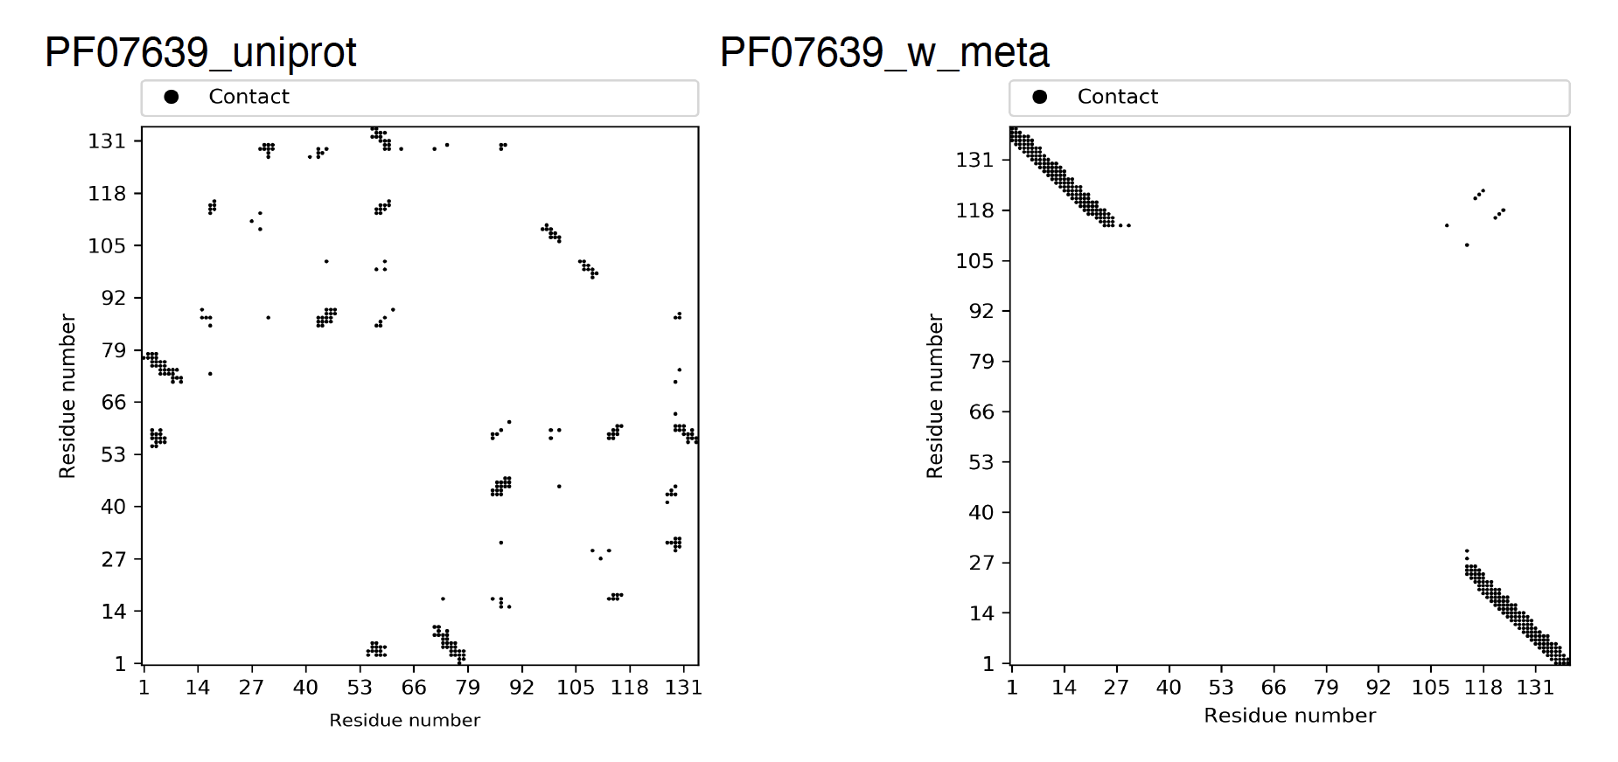
\includegraphics[width=\textwidth]{Experimental Methods/Screenshot 2022-08-02 at 12.14.54.png}
    \caption{Comparison of contact maps constructed with (right) and without (left) metagenomic sequence data.}
    \label{fig:cmap_degrade}
    \small
    Contact were derived using DeepMetaPsicov with the representative sequence for the Pfam domain PF07639.
\end{figure}

Additionally, the use of a metagenomic database made it difficult to maintain annotations as they lack reliable source organism information therefore making the use of phylogeny to link structure to function more difficult.  Therefore any use of metagenomics was considered carefully before implementation.

Results chapters 3 and 4 describe the structure-function investigation into two different autophagy proteins.  Chapter 5 describes the search for specific structural motifs from a number of structural databases.  Methods utilised that were common to more than one chapter are described here with chapter specific methods detailed in the relevant chapter.

Local installations and runs were made on a Ubuntu 18.04.6 workstation  AMD Ryzen Threadripper 2990WX 32 Core CPU (3.0GHz, 80MB CACHE). 64GB Corsair VENGEANCE DDR4 2933MHz ~ (8 x 8GB) was installed.  GPU acceleration was not used for the earlier model building and the graphic card installed was a PNY QUADRO P620 - 2GB GDDR5, 512 CUDA Cores - 4 x mDP.  The required databases were located over two 4TB SEAGATE BARRACUDA SATA-III 3.5" HDD, 6GB/s, 5400RPM, 256MB CACHE.

Model building for the Oca2 protein utilised a local instalation of ColabFold and exploited GPU acceleration via the ASUS TUF GeForce RTX 3080 OC LHR 12GB GDDR6X Ray-Tracing Graphics Card, 8960 Core, 1815MHz Boost.

\section{Software}

\subsection{Pfam Database Screening}
In order to screen the Pfam database with query sequences the HMM-HMM comparison tool, HHpred \cite{El-Gebali2019} (Homology detection and structure prediction by HMM-HMM comparison) was used. HHpred utilises Hidden Markov Models (HMMs) and compares a query protein sequence against a database of profile Hidden Markov Models. HHpred generates a profile Hidden Markov Model from the query sequence. This profile HMM captures the statistical properties and patterns of the query sequence.  HHpred searches a database of profile HMMs, such as the Pfam.  It compares the profile HMM of the query sequence against the profile HMMs in the database.  HHpred performs a sequence-sequence alignment between the query sequence and the database sequences that show significant similarity based on the profile HMM comparison. HHpred then calculates consensus alignments and generates alignment scores, such as the E-value (expectation value - is a statistical measure that estimates the number of false positives expected to be found by chance in a database search; the lower the more significant) and probability score, to assess the significance of the matches. These scores indicate the likelihood of homology and similarity between the query sequence and the matched protein structures. Typical threshold values for probability in HHpred range from 90\% to 95\%, meaning that only matches with a probability above the specified threshold are considered significant.
The threshold for the E-value is typically set to a small value, such as 0.01 or 0.05, implying that only matches with E-values below the threshold are considered significant.

Sequence based searches against the PDB and Pfam-A\_v32.0  databases used the locally installed HHPred v3.0 \cite{Zimmermann2018} with default parameters and eight iterations for MSA generation in the HHblits \cite{Remmert2012} stage;

\begin{lstlisting}[style=linux-terminal]
hhblits -p 20 -Z 10000 -loc -z 1 -b 1 -B 10000 -ssm 2 -sc 1 -seq 1 -dbstrlen 10000 -norealign -maxres 32000 -contxt /path/to/context\_data.crf
\end{lstlisting}

\subsection{Contact map predictions (Metagenomic)}
The MSAs were generated using Jackhmmer v3.3 \cite{Johnson2010}, default parameters with five iterations against a custom metagenomic database. The metagenomic database was a concatenation of: EupathDB \cite{Aurrecoechea2017}, Uniref100 \cite{Apweiler2004}, the Marine Eukaryotic Reference Catalogue (MERC) \cite{Steinegger2018}, the Soil Reference Catalogue (SRC) \cite{Steinegger2018}, MGnify \cite{Mitchell2019}. Local installations of DeepMetapsicov v1.0  \cite{Kandathil2019} and ResPre \cite{Li} were used to generate contact predictions with ConKit v0.12 \cite{conkit2017} utilised to visualise the contact maps. ConPlot was used to overlay additional prediction data \cite{sanchez2021conplot}.

\subsection{Model Building}
\subsubsection{Model building: Rosetta Ab initio}
Rosetta version 3.10 suite \cite{raman2009structure} was used for the initial Roestta model building. Rosetta uses the distribution of local structures in related sequences of solved structures to approximate structures of fragments in the query protein. These short structures are then assembled via a Monte Carlo search with a scoring function based on conformational statistics; Rosetta energy function.  The Rosetta energy function is derived from statistical analysis of known protein structures and incorporates various terms to estimate the energy associated with different aspects of protein conformation, such as bond lengths, angles, and non-bonded interactions \cite{baker2001protein}. 

The Rosetta flag file contains the paths for the fasta sequence, the PSIPRED \cite{McGuffin2000} secondary structure prediction, 3mer/9mer fragments, and the restraint files.

Fragments for the Rosseta Ab initio model building were generated using the local installation of Rosetta Fragment Picker:

\begin{lstlisting}[style=linux-terminal]
/path/to/fragment_picker.linuxgccrelease @best-frags.flags -in::file::vall /path/to/vall.apr24.2008.extended.gz
\end{lstlisting}

Restraint files were generated using python scripts available with the Rosetta distribution; 'create\_evfold\_contact\_map.py' converts contact data (in EVfold \cite{braun2015combining}) to a compatible format that is acceptable c to 'extract\_top\_cm\_restraints.py' \cite{braun2015combining} to create a '.cst' file.  The '.cst' file lists predicted distances generated from the contact data that is used by Rosetta to read and implement the restraints.

\begin{lstlisting}[style=linux-terminal]
/path/to/AbinitioRelax.linuxgccrelease @/flags_tmem41b
\end{lstlisting}


\subsubsection{Model building: RosettaMembrane}
The RosettaMembrane protocol \cite{yarov2006multipass} uses, in addition to the fasta sequence, PSIPRED secondary structure prediction \cite{McGuffin2000}, 3er/9er fragments, and the restraint files, a membrane topology prediction file.  An OCTOPUS \cite{Viklund2008} prediction file is processed using the 'octopus2span.pl' Perl script.  The output file is then further processed into a format acceptable to RosettaMembrane using the 'run\_lips.pl' script;

\begin{lstlisting}[style=linux-terminal]
/path/to/run_lips.pl ../tmem41b.fasta ./tmem41b.span /path/to/blastpgp /db_blast/nr /path/to/alignblast.pl
\end{lstlisting}


The script did have to be modified due to it attempting to run a CGI script (lips.txt) that was no longer available remotely; the url is not run as a CGI (Common Gateway Interface) script, it was just where the script could be downloaded from. A CGI  script allows interaction between a web server and other software applications, enabling dynamic content generation and processing of user requests. CGI scripts are commonly used to perform tasks such as processing form data and interacting with databases. When a user submits a request to a web server, the server can execute a CGI script to process the request and generate a response. The CGI script can receive input parameters from the user's request, perform necessary computations or operations, and generate an output. In this case as the CGI script was no longer available the script was run locally by downloading (http://tanto.bioe.uic.edu/lips/lips.txt), made executable and the run\_lips.pl was made to point at the local script rather than the url by modifying line 132 in order to execute the local version of the script;

\begin{lstlisting}[style=linux-terminal]
$data=`curl -s $url -d sequence='$sequences' -d num=$first_num`;
\end{lstlisting}
to \\

\begin{lstlisting}[style=linux-terminal]
$data=`/rosetta/lips.txt -d sequence='$sequences' -d num=$first_num`;
\end{lstlisting}

The RosettaMembrane is then executed with the appropriate flag file;

\begin{lstlisting}[style=linux-terminal]
/path/to/membrane_abinitio2.linuxgccrelease @ ./flags_membrane.txt
\end{lstlisting}

\subsubsection{Clustering of Rosetta Decoys}
SPICKER \cite{Zhang2004} (SPatial Clustering with Kernels) is a protein structure clustering algorithm used to group similar protein structures based on their three-dimensional coordinates. SPICKER takes a set of protein structures as input, typically represented by their Cartesian coordinates (x, y, z) of atoms. SPICKER then calculates the pairwise root-mean-square deviation (RMSD) distances between all pairs of structures. RMSD measures the structural similarity between two protein structures by quantifying the average distance between corresponding atoms after superimposition. SPICKER employs a kernel density estimation technique to estimate the density of structures in the multi-dimensional RMSD space. It constructs a density function by assigning each structure a probability density value based on its RMSD distance to other structures.v The density-based clustering algorithm DBSCAN (Density-Based Spatial Clustering of Applications with Noise) is applied to identify clusters in the estimated density function. DBSCAN groups structures that have high density and are closely located in the RMSD space. Structures that are not in any cluster are considered as noise.  SPICKER selects the most representative structure from each cluster based on the average RMSD distance to other structures in the same cluster. This representative structure is often referred to as a "centroid" or "medoid" and is used to represent the cluster.

SPICKER \cite{Zhang2004} was used to cluster the output models from Rosetta.  SPICKER was executed within the ccp4 suite which auto generates the required input files.

\begin{lstlisting}[style=linux-terminal]
ccp4-python /path/to/spicker.py -e /path/to/spicker -m ./models/ -t 50 
\end{lstlisting}



\subsubsection{Model building: trRosetta}
Ab initio models were built using the trRosetta \cite{Yang2020} local installation with default settings utilising an MSA from HHblits in the '.a3m' format. Transform-restrained Rosetta (trRosetta) is a Rosetta protocol that utilises predicted distances and orientations as restraints that are derived from a deep residual-convolutional network.  The network takes an MSA as input and the outputs are used as energy minimisation restraints in the Rosetta model building.  This differs from Rosetta contact assisted ab initio model building as in addition to the C$\beta$–C$\beta$ distances the orientations (defined by six parameters) are predicted which accurately describe the relative positions of the backbone of two residues.

The predicted distances and side-chain orientations were generated using:
\begin{lstlisting}[style=linux-terminal]
python ./predict.py -m ./model2019 example/T1001.a3m example/T1001.npz
\end{lstlisting}
Models are constructed using trRosetta by:
\begin{lstlisting}[style=linux-terminal]
python trRosetta.py T1008.npz T1008.fasta model.pdb
\end{lstlisting}

\subsubsection{Model building: DMPfold}
DMPfold \cite{Greener2019} utilises deep-learning to predict inter-residue distances, main chain hydrogen bond network and torsion angles.  These are then used in the model building process. The Ab initio models were built using a DMPfold local installation with default settings utilising an MSA built by Jackhmmer.  The alignments in '.aln' format is then used by a DMPfold script to generate distance restraints: 
\begin{lstlisting}[style=linux-terminal]
csh aln2maps.csh example/PF10963.aln
\end{lstlisting}
The restraints were then used to build the models:
\begin{lstlisting}[style=linux-terminal]
/path/to/DMPfold/run_dmpfold.sh /w9dy28.fasta ../output.21c ../output.map ./w9_1_84_models
\end{lstlisting}

\subsubsection{Homology Modelling}
Homology modeling, also known as comparative modeling, is a computational method used to predict the three-dimensional structure of a protein based on its sequence similarity to one or more known protein structures. It relies on the principle that proteins with high sequence similarity share similar structures and functions. A target protein, is selected for which the experimental structure is unknown but a related template structure with known three-dimensional coordinates exists. Suitable template structures are identified by searching sequence databases using algorithms such as HHpred. Templates with high sequence similarity to the target are preferred, ideally with sequence identity above a certain threshold (e.g., 30-40\%). The target protein sequence is aligned with the template sequence to identify corresponding positions and regions. Using the sequence alignment as a guide, the three-dimensional coordinates of the target protein are constructed by copying the coordinates from the template structure. The quality and reliability of the homology model are assessed using various validation criteria and scoring functions. This study employed predicted contact satisfaction scores (see below). MODELLER \cite{eswar2006comparative} is a software package widely used for homology modeling and comparative protein structure prediction and was used for the study of Atg9 (Chapter 4). 

\subsection{Transmembrane Region Prediction}
Unless otherwise stated the transmembrane helical topology predictions were obtained from the Topcons server \cite{Tsirigos2015}. TopCons combines multiple sources of information, including predicted transmembrane helices, signal peptides, and homologous proteins, to make accurate predictions.  Based on this combined information from signal peptide prediction, transmembrane helix prediction, and homology-based prediction, TopCons generates a consensus prediction for the presence and location of transmembrane regions in the protein sequence.

When confidence scores were required for individual transmembrane region predictions TMHMM (TransMembrane Hidden Markov Model) was employed. TMHMM employs a Hidden Markov Model (HMM) approach.  TMHMM is trained using a dataset of known transmembrane proteins with experimentally verified transmembrane helices. The HMM is trained to recognize the statistical patterns and properties associated with transmembrane regions.

Other transmembrane prediction software was utilised for comparison purposes:
\begin{enumerate}
\item Octopus \cite{viklund2008octopus};
\item Spoctopus \cite{teixeira2017membrane}; 
\item Philius \cite{reynolds2008transmembrane} ;
\item Polyphobius \cite{jones2007improving} ;
\item SCAMPI \cite{reeb2015evaluation};
\end{enumerate}

\subsection{Secondary Structure Prediction}
Secondary structure predictions were made employing a local installation of PSIPRED v4.0 \cite{McGuffin2000}. (Protein Structure Prediction Server). PSIPRED employs a  neural network to make its predictions. PSIPRED Generates a position-specific scoring matrix (PSSM). A PSSM is a matrix that encodes the sequence profile, which represents the frequency and propensity of each amino acid at each position in the sequence. The PSSM is generated by performing a sequence database search using tools like PSI-BLAST \cite{altschul1998iterated}. The final output of PSIPRED is a prediction of the secondary structure for each residue in the protein sequence. This prediction is usually represented as a sequence of letters corresponding to the predicted secondary structure states (H for alpha helix, E for beta strand, and C for coil).

\subsection{Conservation Mapping}
Conservation was mapped on to the models using the ConSurf server \cite{Ashkenazy2016}. 

To visualise the conservation as a spectrum using Consurfs conventional spectrum the Consurf processed PDB file (with updated with ConSurf colours - PDB\_FILE) and the python script, consurf\_new.py, was downloaded from the server; PyMol was then initialised and the processed PDB file was loaded with the subsequent run of the consurf\_new.py script ('run consurf\_new.py' in PyMol terminal);


\subsection{Visualisation of Models}
Visualisation of models was achieved using PyMOL v2.3.0 \cite{DeLano2002}.

Membrane planes were visualised by:

\begin{enumerate}
\item Downloading membrane\_planes.py \cite{baugh2011real} from RosettaCommons and place in the same directory as the PyMol executable;
\item Downloading visualise\_membranes.pml from RosettaCommons the attached .pml \cite{baugh2011real} file;
\item Download the translated version of the pdb file from PDBTM or generate the translated version from the OPM server; 
\item Initialise pymol with a command like the following;  
\begin{lstlisting}[style=linux-terminal]
/path/to/PyMOL ./3org.pdb ./visualize_membrane.pml  (/path/to/pymol/executable/ /path/to/translated/pdb/file/ /path/to/pml/file)
\end{lstlisting}

\end{enumerate}

\subsection{Structural Alignments}
Structural alignment methods aim to compare and align protein structures to identify similarities, infer evolutionary relationships, and gain insights into their functional and structural properties. There are many methods for assessing similarity \cite{Holm2016,orengo199636,falicov1996surface,krissinel2004secondary} and commonly rely on comparing the sizes of shared substructures, such as the length of alignment, where longer alignments are considered more favorable. Additionally, a distance measure like RMSD (Root Mean Square Deviation) is commonly used to evaluate the difference between these substructures, with lower values indicating greater similarity.  RMSD  quantifies the average distance between corresponding atoms in the two sets of coordinates. It is calculated by aligning the structures and measuring the displacement of each atom.  The distance between each pair of corresponding atoms in the superposed structures is calculated. The deviation or displacement of each atom is obtained by subtracting the position of the corresponding atom in one structure from the position of the corresponding atom in the other structure. The deviations are squared, and the squared deviations are summed across all atoms in the structure. The summed squared deviations are divided by the number of atoms, and the square root of the result is taken to obtain the RMSD value \cite{yusuf2008alternative}.  

\[ \text{RMSD} = \sqrt{\frac{\sum\limits_{i=1}^{n}(x_i - y_i)^2}{n}} \]

\begin{itemize}
\item  \(N\) is the total number of atoms.
\item  \(\mathbf{X}_i\) and \(\mathbf{Y}_i\) denote the coordinates of the corresponding atoms in the two compared structures.
\item  The summation \(\sum_{i=1}^{N}\) iterates over all the atoms.
\item  \((\mathbf{X}_i - \mathbf{Y}_i)^2\) calculates the squared differences between the corresponding atom coordinates.
\end{itemize}
RMSD is expressed in units of length. A lower RMSD value indicates a closer match between the structures, while a higher RMSD value suggests greater differences or structural variation.

Local installation of Dali v4.0 \cite{Holm2016} was used to structurally align the output models and to query against the PDBTM \cite{Kozma2012}.  Dali has high sensitivity in detecting structural similarities identifying remote homologues and recognise similarities even when sequence similarity is low.  Dali is capable of handling both small and large protein structures and can align multiple structures simultaneously, enabling the detection of structural relationships among a set of proteins.  Dali provides Z-scores that assess the significance of the structural similarity. This statistical measure helps evaluate the reliability of the alignments and distinguish true similarities from random matches. Z-scores provide a measure of how well the observed similarity score (DALI Z-score) compares to the scores obtained from random structure alignments.  First Dali generates random structural alignments by shuffling and superimposing the secondary structure elements of the two proteins being compared. This generates a distribution of similarity scores for random alignments.  The similarity score used in Dali is the Z-score-like score, which is based on the root mean square deviation (RMSD) between aligned residues, the number of aligned residues, and the length of the proteins. The Z-score is then calculated by comparing the similarity score of the observed alignment with the distribution of scores obtained from the random alignments. It represents the number of standard deviations the observed score is away from the mean of the random distribution. A higher Z-score indicates a higher level of significance for the structural similarity.


\subsection{Precision}
Precision score evaluation of models in relation to the predicted contacts at various contact cutoff values were calculated and plotted using ConKit. A 70\% precision cut off  for the top L contacts is suggestive of good quality models \cite{DeOliveira2016}.
%where L = sequence length (rounded down to the nearest whole number of contacts)


\subsection{Other prediction data}
ConKit was also used to predict and visualise potential structural domain boundaries \cite{Rigden2002}\cite{Simkovic2017}. Residue analysis of putative amphipathic regions were performed using HELIQUEST \cite{Gautier2008} to determine the presence, direction and magnitude of any hydrophobic moment. 
